\documentclass[conference]{IEEEtran}
\usepackage[utf8]{inputenc}
\usepackage[T1]{fontenc}
\usepackage{amsmath,amssymb}
\usepackage{graphicx}
\usepackage{booktabs}
\usepackage{array}
\usepackage{xcolor}
\usepackage{url}
\usepackage{tikz}
\usetikzlibrary{positioning,arrows.meta,fit,calc}
\usepackage{pgfplots}
\pgfplotsset{compat=1.17}
\usepgfplotslibrary{groupplots,statistics}
\usepackage{balance}
\usepackage[hidelinks]{hyperref}

\newcommand{\code}[1]{\texttt{#1}}

\begin{document}

\title{CogniHire: Auditing R\'esum\'e Claims Instead of\\Scoring Candidates}

\author{\IEEEauthorblockN{Devesh S V}
\IEEEauthorblockA{Department of Computer Science and Engineering\\
SRM Institute of Science and Technology\\
Chennai, India\\
deveshsv.386@gmail.com}}

\maketitle

\begin{abstract}
Automated hiring systems overwhelmingly emit a \emph{score}: a scalar that
ranks a candidate against others. Such scores resist explanation, give a
candidate nothing specific to contest, and carry growing regulatory exposure
under New York City Local Law~144, the Illinois Human Rights Act as amended by
HB~3773, and the EU Artificial Intelligence Act. We present CogniHire, a
technical screening system built on the opposite premise: it audits the claims
a candidate makes and never scores the candidate. Three technology families
carry the load. Evidence grounding constrains a language model to \emph{select}
claim text and forbids it to \emph{author} any; across roughly 100,000
adversarial trials over 5,200 r\'esum\'es the gate rejected every
meaning-preserving paraphrase and every negation trap while admitting every
verbatim claim. For machine learning we report a nine-model, six-family
comparison under grouped cross-validation with significance testing, and a
within-query diagnostic that separates matching ability from candidate-level
quality, which pooled metrics cannot do. For deep learning we show that a
plausible authored face-similarity threshold of 0.50 would have falsely
rejected 41.4\% of genuine identity matches, against 3.4\% at a threshold
calibrated on Labeled Faces in the Wild. The recurring engineering move is
converting policy into structure: an import boundary that fails the build, a
type with no field to hold a fabricated value, a vocabulary ban that forbids a
composite score.
\end{abstract}

\begin{IEEEkeywords}
automated hiring, evidence grounding, claim verification, algorithmic
accountability, model comparison, face verification, threshold calibration
\end{IEEEkeywords}

% ---------------------------------------------------------------- Fig. 1
\begin{figure}[t]
\centering
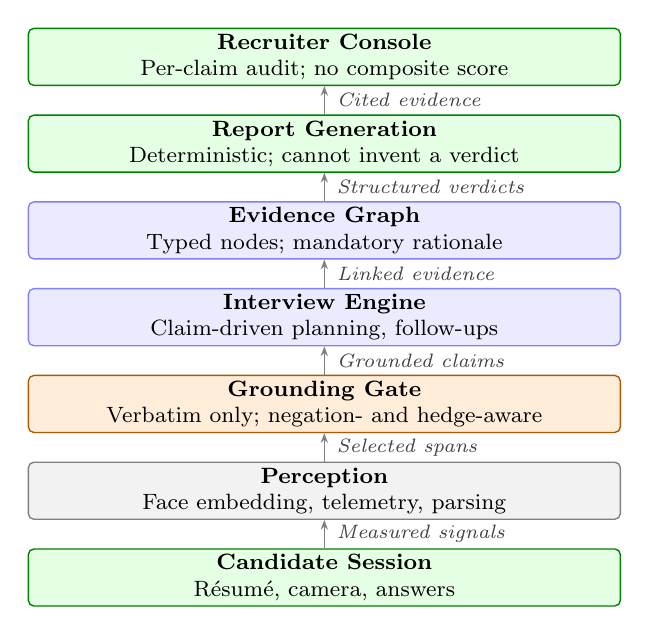
\begin{tikzpicture}[
  layer/.style={draw, rounded corners=2pt, minimum width=0.62\columnwidth, minimum height=0.72cm,
                align=center, font=\footnotesize, line width=0.5pt, inner sep=2pt},
  flow/.style={-{Stealth[length=3.5pt]}, gray},
  lbl/.style={font=\scriptsize\itshape, text=black!75, anchor=west},
  node distance=0.36cm]
\node[layer, fill=green!10, draw=green!50!black] (cs) {\textbf{Candidate Session}\\R\'esum\'e, camera, answers};
\node[layer, fill=gray!10, draw=gray, above=of cs] (pe) {\textbf{Perception}\\Face embedding, telemetry, parsing};
\node[layer, fill=orange!15, draw=orange!70!black, above=of pe] (gg) {\textbf{Grounding Gate}\\Verbatim only; negation- and hedge-aware};
\node[layer, fill=blue!8, draw=blue!50, above=of gg] (ie) {\textbf{Interview Engine}\\Claim-driven planning, follow-ups};
\node[layer, fill=blue!8, draw=blue!50, above=of ie] (eg) {\textbf{Evidence Graph}\\Typed nodes; mandatory rationale};
\node[layer, fill=green!10, draw=green!50!black, above=of eg] (rg) {\textbf{Report Generation}\\Deterministic; cannot invent a verdict};
\node[layer, fill=green!10, draw=green!50!black, above=of rg] (rc) {\textbf{Recruiter Console}\\Per-claim audit; no composite score};
\foreach \a/\b/\t in {cs/pe/Measured signals, pe/gg/Selected spans, gg/ie/Grounded claims,
                      ie/eg/Linked evidence, eg/rg/Structured verdicts, rg/rc/Cited evidence}{
  \draw[flow] (\a.north) -- (\b.south) node[midway, lbl, xshift=1pt] {\t};
}
\end{tikzpicture}
\caption{Data flow in CogniHire. Evidence moves upward from the candidate
session to the recruiter console; each transition narrows what the system may
assert. The guarantees enforced at these boundaries are listed in
Table~\ref{tab:policies}.}
\label{fig:flow}
\end{figure}

\section{Introduction}
A technical interview ends and a form is filled in: \emph{``Strong
communication. Good Flutter knowledge. 8.7/10.''} Six months later the number
is indefensible. Nobody can reconstruct which answer moved it from 8.4 to 8.7;
the candidate cannot appeal it and the recruiter cannot defend it. The number
was a compression of knowledge that discarded everything needed to audit it.

Automated interview platforms largely reproduce this failure at scale. Faced
with criticism, the industry has made the scalar more sophisticated---more
features, better models, fairness post-processing---but few have asked whether
a scalar was the right output object at all.

We take the opposite position: the useful output of automated screening is an
audit of the claims a candidate has made, not a judgment of the candidate. A
r\'esum\'e is a set of assertions. Each can be probed, each probe yields
evidence, and evidence supports a verdict about \emph{the claim}. The verdicts,
with evidence attached, go to a human who decides about \emph{the person}
(Fig.~\ref{fig:flow}). This changes what the system must be \emph{unable} to
do, and which technology belongs at which layer: grounding governs what may be
asserted, machine learning (ML) measures properties of evidence, and deep
learning (DL) supplies perception.

Our contributions are:
\begin{enumerate}
\item A \textbf{claim-audit output model} replacing the composite score, with a
  four-valued verdict set that makes unmeasured evidence explicit.
\item A \textbf{structurally enforced grounding constraint}, measured at 100\%
  paraphrase and negation-trap rejection over ${\sim}$100,000 trials.
\item A \textbf{nine-model comparison} under grouped cross-validation with
  Friedman and Holm-corrected Wilcoxon tests, plus a synthetic positive control
  establishing statistical power.
\item A \textbf{within-query ranking diagnostic} that separates matching from
  entity-level quality on any paired benchmark.
\item An \textbf{empirical threshold calibration} showing that a documented,
  authored constant was wrong by a quantified amount.
\end{enumerate}

\section{Related Work}
Raghavan et al.~\cite{raghavan2020} surveyed vendors of algorithmic
pre-employment assessment and highlighted the consequences of a vendor's choice
of prediction target: fairness analysis is conducted against the stated target
rather than the deployed one. They offer no remedy for a misdescribed target;
Section~\ref{sec:within} supplies a measurement that detects one.

A second strand re-ran published comparisons under controlled protocols.
Ferrari Dacrema et al.~\cite{dacrema2019} could reproduce only seven of
eighteen neural recommenders, six of which were often beaten by simple
heuristics; Musgrave et al.~\cite{musgrave2020} found the same for deep metric
learning, and Grinsztajn et al.~\cite{grinsztajn2022} showed tree ensembles
still rival deep networks on tabular data. We differ in finding that no method
separates from any other, and then tracing why.

On evaluation protocol, Dem\v{s}ar~\cite{demsar2006} cautions against reading a
ranking off raw score differences; Nadeau and Bengio~\cite{nadeau2003} show
that overlapping training sets bias naive variance estimates; Gorman and
Bedrick~\cite{gorman2019} showed rankings from a single standard split often
fail to reproduce; and Kapoor and Narayanan~\cite{kapoor2023} documented
leakage in 294 ML-based science papers. We adopt Dem\v{s}ar's protocol and
quantify one leakage category on a hiring benchmark.

For perception we build on SCRFD~\cite{guo2022} and ArcFace~\cite{deng2019},
which leave the verification threshold to the integrator, and calibrate it on
LFW~\cite{huang2007}. Across these strands three gaps recur: no work
constrains generative extraction to selection; prediction targets go
unverified behind pooled metrics; and perception components ship with
authored, unmeasured thresholds.

\begin{table}[t]
\caption{Policies Converted Into Structural Guarantees}
\label{tab:policies}
\centering
\footnotesize
\begin{tabular}{@{}>{\raggedright\arraybackslash}p{0.40\columnwidth}>{\raggedright\arraybackslash}p{0.53\columnwidth}@{}}
\toprule
Policy & Structure \\
\midrule
AI must not author claims & Import boundary plus a CI architecture test \\
Unmeasured is not passed & Result type with no similarity field \\
No composite score & Vocabulary ban that fails the build \\
No demographic inference & Classifier module never loaded (allow-list) \\
No outcome labels & No such dataset, no code path to build one \\
Plans cannot be edited later & Question plans never persisted \\
Sessions reconstructible & Append-only event table with sequencing trigger \\
\bottomrule
\end{tabular}
\end{table}

\section{System Architecture}
CogniHire spans four surfaces: a candidate portal (consent, r\'esum\'e, session
media), an inference service (perception and learned components), an
event-sourced persistence layer, and a recruiter console that renders the
audit. Every guarantee is enforced at a boundary between two surfaces. Session
state is written to an append-only table with a sequence-assigning trigger, so
a session can be reconstructed turn by turn; question plans are never
persisted, so a plan cannot be edited after the fact to match an outcome.

The audit has four verdicts:
\begin{itemize}
\item \code{substantiated},
\item \code{notDemonstrated},
\item \code{contradicted}, and
\item \code{notExamined}.
\end{itemize}
The four are deliberately not
orderable, and no composite is computed. \code{notExamined} is load-bearing:
without it an unprobed claim is simply absent from the report, and absence
reads as acceptance.

Table~\ref{tab:policies} lists the policies the system converts into
structures. Each turns a claim that requires trust into one a skeptical
reviewer can check by inspection.

\section{Evidence Grounding}
\subsection{The Grounding Gate}
The central rule: a claim's text must be a verbatim substring of the
r\'esum\'e. The model selects; it does not generate. Naive substring matching
is insufficient, so the gate (Fig.~\ref{fig:gate}) adds negation rejection
(``I have not worked with Kubernetes'' yields no Kubernetes claim), hedge
rejection (``some exposure to Kafka''), contrastive-conjunction splitting (``I
used Django, but never in production''), and clause scoping, so matching never
crosses a clause boundary.

\begin{figure}[t]
\centering
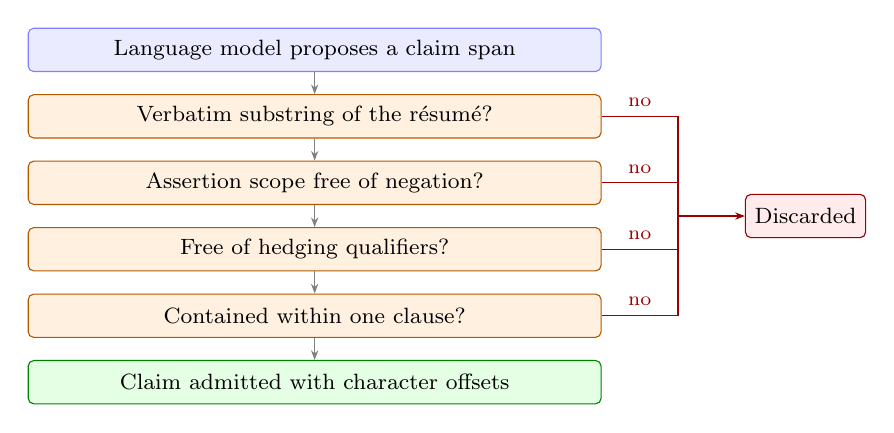
\begin{tikzpicture}[
  gstep/.style={draw=orange!70!black, fill=orange!12, rounded corners=2pt, minimum width=0.60\columnwidth,
               minimum height=0.55cm, font=\footnotesize, align=center},
  io/.style={gstep, draw=blue!50, fill=blue!8},
  ok/.style={gstep, draw=green!50!black, fill=green!10},
  arr/.style={-{Stealth[length=3.5pt]}, gray},
  node distance=0.28cm]
\node[io] (in) {Language model proposes a claim span};
\node[gstep, below=of in] (q1) {Verbatim substring of the r\'esum\'e?};
\node[gstep, below=of q1] (q2) {Assertion scope free of negation?};
\node[gstep, below=of q2] (q3) {Free of hedging qualifiers?};
\node[gstep, below=of q3] (q4) {Contained within one clause?};
\node[ok, below=of q4] (out) {Claim admitted with character offsets};
\node[draw=red!60!black, fill=red!8, rounded corners=2pt, font=\footnotesize, minimum height=0.55cm,
      anchor=west] (no) at ([xshift=0.15\columnwidth]$(q2.east)!0.5!(q3.east)$) {Discarded};
\coordinate (bus) at ([xshift=0.08\columnwidth]q1.east);
\foreach \a/\b in {in/q1,q1/q2,q2/q3,q3/q4,q4/out} \draw[arr] (\a) -- (\b);
\foreach \q in {q1,q2,q3,q4} \draw[red!60!black] (\q.east) -- node[above, font=\scriptsize, pos=0.5]{no} (\q.east -| bus);
\draw[red!60!black] (q1.east -| bus) -- (q4.east -| bus);
\draw[arr, red!60!black] ($(q2.east -| bus)!0.5!(q3.east -| bus)$) -- (no.west);
\end{tikzpicture}
\caption{The grounding gate as a decision pipeline. Any \emph{no} branch
discards the proposed claim.}
\label{fig:gate}
\end{figure}

The grounding module is forbidden from importing the AI module, and an
architecture test fails continuous integration if that import appears. The
guarantee is a property of the build, not of developer discipline. Because the
planner consumes only typed claims, an instruction embedded in a r\'esum\'e has
no field to occupy, which also closes the prompt-injection channel.

\subsection{Measured Behavior}
An offline deterministic harness drives the real pipeline modules over 5,200
synthetic r\'esum\'es spanning eight fields and four seniority levels. No
language-model key is needed, so the result is reproducible. Across roughly
100,000 trials the gate rejected all 48,149 meaning-preserving paraphrases and
all 51,761 negation traps (Table~\ref{tab:gate}).

\begin{table}[t]
\caption{Grounding-Gate Correct-Decision Rate Before and After the Clause-Splitter Fix}
\label{tab:gate}
\centering
\footnotesize
\begin{tabular}{@{}lrcc@{}}
\toprule
Trial type & $n$ & Before fix & After fix \\
\midrule
Paraphrases (must reject)    & 48,149 & 100\%   & 100\% \\
Negation traps (must reject) & 51,761 & 100\%   & 100\% \\
Verbatim claims (must admit) & 51,761 & 99.18\% & \textbf{100\%} \\
\bottomrule
\end{tabular}
\end{table}

The initial run showed a 0.82\% false-rejection rate: 425 of 51,761 genuine
claims discarded, every one containing a period-bearing token such as
\code{Node.js}, \code{asp.net} or \code{Python~3.9}. The clause splitter treated every period as
a terminal, so ``Node.js.'' split into ``Node'' and ``js.'' and the claim was
\emph{silently} dropped. Requiring a terminal to be followed by whitespace or
end-of-string fixed it; since the change only makes clauses longer, it widens
negation scope and cannot weaken the guard. Verbatim admission rose to 100\%
with both rejection rates unchanged. No unit test caught this defect; only
corpus-scale measurement with an explicit true-positive metric did.

The corpus is synthetic and single-generator, so we do not claim 100\%
extraction coverage in general. The defensible claim concerns the safety
mechanism: the model selects and never authors.

\section{Machine Learning: What Model Choice Buys}
ML in CogniHire measures properties of evidence; it is never trained on hiring
outcomes. To test how much algorithm choice matters in screening, we compared
nine classifiers from six families on a public r\'esum\'e--posting fit
benchmark~\cite{cnamuangtoun2024} of 7,910 balanced pairs (643 r\'esum\'es,
351 postings), using scikit-learn~\cite{pedregosa2011}. The dataset card states
no description, license, or labeling procedure, which bounds how far any
result on it generalizes.

\subsection{Protocol and Results}
Every experiment uses ten-fold \code{GroupKFold} grouped by posting. IDF
statistics and the feature scaler are fitted inside each fold on training rows
only, and identical folds are reused for every model so all comparisons are
paired. Table~\ref{tab:nine} reports the results.

\begin{table}[t]
\caption{Nine Classifiers, Ten-Fold Cross-Validation Grouped by Posting
(Mean $\pm$ Fold Std.)}
\label{tab:nine}
\centering
\footnotesize
\setlength{\tabcolsep}{4pt}
\begin{tabular}{@{}lcccr@{}}
\toprule
Model & AUROC & ECE & Lat.\ ($\mu$s) & Size (KB) \\
\midrule
MLP                 & \textbf{0.696 $\pm$ 0.031} & 0.057 & 0.5   & 74.7 \\
Gradient boosting   & 0.689 $\pm$ 0.028 & 0.047 & 1.9   & 393.3 \\
Random forest       & 0.688 $\pm$ 0.030 & 0.047 & 88.2  & 24,732.6 \\
SVM (RBF)           & 0.686 $\pm$ 0.028 & 0.053 & 195.0 & 526.8 \\
Extra trees         & 0.685 $\pm$ 0.030 & \textbf{0.046} & 84.9 & 63,415.9 \\
$k$-NN              & 0.680 $\pm$ 0.031 & 0.057 & 35.5  & 1,272.8 \\
Hist.\ grad.\ boosting & 0.679 $\pm$ 0.029 & 0.057 & 7.3   & 591.8 \\
Gaussian NB         & 0.667 $\pm$ 0.033 & 0.117 & 0.3   & 1.1 \\
Logistic regression & 0.665 $\pm$ 0.022 & 0.052 & \textbf{0.2} & \textbf{0.9} \\
\bottomrule
\end{tabular}
\end{table}

The nine span only 0.031 AUROC, comparable to each model's fold-to-fold
standard deviation. The Friedman test rejects identical performance
($\chi^2 = 38.35$, $p = 6.5\times10^{-6}$), but under paired Wilcoxon tests
with Holm correction the leading MLP is \textbf{statistically
indistinguishable from all four tree ensembles}. A ranked table alone would
have licensed ``MLP is best''; the significance analysis does not.

\emph{Power.} A null is uninformative unless the protocol can detect a
difference when one exists. On a synthetic control with a planted generative
process (Bayes-optimal accuracy 0.925), the same nine models under the
identical code path separate decisively ($\chi^2 = 55.42$,
$p = 3.7\times10^{-9}$; Fig.~\ref{fig:folds}). The null is a property of the
task, not the protocol.

\begin{figure*}[t]
\centering
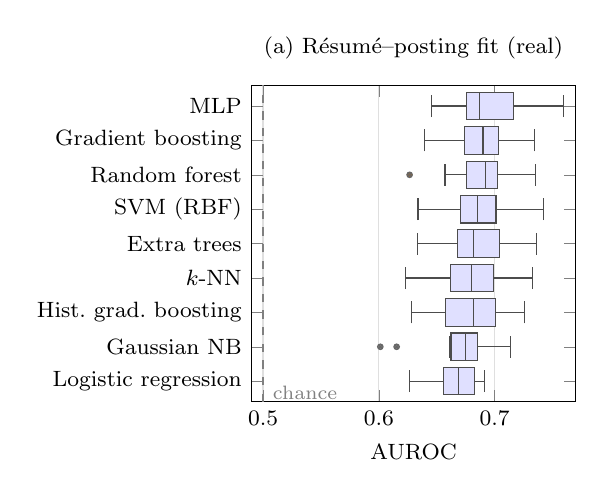
\begin{tikzpicture}
\begin{axis}[boxplot/draw direction=x, clip=false, width=0.47\textwidth, height=5.6cm, ytick={9,8,7,6,5,4,3,2,1}, ymin=0.4, ymax=9.6, ticklabel style={font=\footnotesize}, label style={font=\footnotesize}, title style={font=\footnotesize}, xmajorgrids, grid style={gray!25}, mark options={mark size=1pt, black!60}, yticklabels={{MLP},{Gradient boosting},{Random forest},{SVM (RBF)},{Extra trees},{$k$-NN},{Hist.\ grad.\ boosting},{Gaussian NB},{Logistic regression}}, xmin=0.49, xmax=0.77, xlabel={AUROC}, title={(a) R\'esum\'e--posting fit (real)},
  xticklabel style={/pgf/number format/fixed, /pgf/number format/precision=2}]
\draw[dashed, gray] (axis cs:0.5,0.4) -- (axis cs:0.5,9.6) node[pos=0.03, right, font=\scriptsize, text=gray] {chance};
\addplot+[boxplot prepared={draw position=9,lower whisker=0.6456,lower quartile=0.6756,median=0.6870,upper quartile=0.7162,upper whisker=0.7592},draw=black!70,fill=blue!12,solid] coordinates {};
\addplot+[boxplot prepared={draw position=8,lower whisker=0.6392,lower quartile=0.6740,median=0.6900,upper quartile=0.7030,upper whisker=0.7343},draw=black!70,fill=blue!12,solid] coordinates {};
\addplot+[boxplot prepared={draw position=7,lower whisker=0.6572,lower quartile=0.6759,median=0.6921,upper quartile=0.7023,upper whisker=0.7350},draw=black!70,fill=blue!12,solid] coordinates {(0,0.6266)};
\addplot+[boxplot prepared={draw position=6,lower whisker=0.6338,lower quartile=0.6706,median=0.6852,upper quartile=0.7012,upper whisker=0.7420},draw=black!70,fill=blue!12,solid] coordinates {};
\addplot+[boxplot prepared={draw position=5,lower whisker=0.6333,lower quartile=0.6680,median=0.6816,upper quartile=0.7039,upper whisker=0.7364},draw=black!70,fill=blue!12,solid] coordinates {};
\addplot+[boxplot prepared={draw position=4,lower whisker=0.6232,lower quartile=0.6622,median=0.6799,upper quartile=0.6991,upper whisker=0.7325},draw=black!70,fill=blue!12,solid] coordinates {};
\addplot+[boxplot prepared={draw position=3,lower whisker=0.6281,lower quartile=0.6575,median=0.6814,upper quartile=0.7011,upper whisker=0.7261},draw=black!70,fill=blue!12,solid] coordinates {};
\addplot+[boxplot prepared={draw position=2,lower whisker=0.6607,lower quartile=0.6623,median=0.6748,upper quartile=0.6849,upper whisker=0.7141},draw=black!70,fill=blue!12,solid] coordinates {(0,0.6154) (0,0.6013)};
\addplot+[boxplot prepared={draw position=1,lower whisker=0.6262,lower quartile=0.6562,median=0.6689,upper quartile=0.6824,upper whisker=0.6912},draw=black!70,fill=blue!12,solid] coordinates {};
\end{axis}
\end{tikzpicture}\hfill
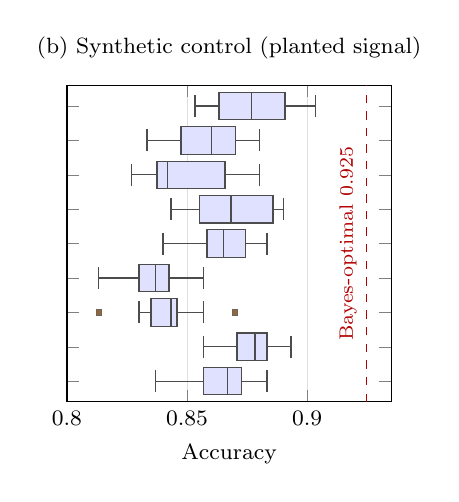
\begin{tikzpicture}
\begin{axis}[boxplot/draw direction=x, clip=false, width=0.47\textwidth, height=5.6cm, ytick={9,8,7,6,5,4,3,2,1}, ymin=0.4, ymax=9.6, ticklabel style={font=\footnotesize}, label style={font=\footnotesize}, title style={font=\footnotesize}, xmajorgrids, grid style={gray!25}, mark options={mark size=1pt, black!60}, yticklabels={}, xmin=0.80, xmax=0.935, xlabel={Accuracy}, title={(b) Synthetic control (planted signal)},
  xticklabel style={/pgf/number format/fixed, /pgf/number format/precision=2}]
\draw[dashed, red!70!black] (axis cs:0.9247,0.4) -- (axis cs:0.9247,9.6) node[pos=0.5, rotate=90, anchor=south, font=\scriptsize, text=red!70!black] {Bayes-optimal 0.925};
\addplot+[boxplot prepared={draw position=9,lower whisker=0.8533,lower quartile=0.8633,median=0.8767,upper quartile=0.8908,upper whisker=0.9033},draw=black!70,fill=blue!12,solid] coordinates {};
\addplot+[boxplot prepared={draw position=8,lower whisker=0.8333,lower quartile=0.8475,median=0.8600,upper quartile=0.8700,upper whisker=0.8800},draw=black!70,fill=blue!12,solid] coordinates {};
\addplot+[boxplot prepared={draw position=7,lower whisker=0.8267,lower quartile=0.8375,median=0.8417,upper quartile=0.8658,upper whisker=0.8800},draw=black!70,fill=blue!12,solid] coordinates {};
\addplot+[boxplot prepared={draw position=6,lower whisker=0.8433,lower quartile=0.8550,median=0.8683,upper quartile=0.8858,upper whisker=0.8900},draw=black!70,fill=blue!12,solid] coordinates {};
\addplot+[boxplot prepared={draw position=5,lower whisker=0.8400,lower quartile=0.8583,median=0.8650,upper quartile=0.8742,upper whisker=0.8833},draw=black!70,fill=blue!12,solid] coordinates {};
\addplot+[boxplot prepared={draw position=4,lower whisker=0.8133,lower quartile=0.8300,median=0.8367,upper quartile=0.8425,upper whisker=0.8567},draw=black!70,fill=blue!12,solid] coordinates {};
\addplot+[boxplot prepared={draw position=3,lower whisker=0.8300,lower quartile=0.8350,median=0.8433,upper quartile=0.8458,upper whisker=0.8567},draw=black!70,fill=blue!12,solid] coordinates {(0,0.8133) (0,0.8700)};
\addplot+[boxplot prepared={draw position=2,lower whisker=0.8567,lower quartile=0.8708,median=0.8783,upper quartile=0.8833,upper whisker=0.8933},draw=black!70,fill=blue!12,solid] coordinates {};
\addplot+[boxplot prepared={draw position=1,lower whisker=0.8367,lower quartile=0.8567,median=0.8667,upper quartile=0.8725,upper whisker=0.8833},draw=black!70,fill=blue!12,solid] coordinates {};
\end{axis}
\end{tikzpicture}

\caption{Per-fold results over ten grouped folds. (a) Nine models on the real
screening task (AUROC): boxes overlap almost completely. (b) Same models,
folds, and code on the synthetic positive control (accuracy), which they
separate clearly.}
\label{fig:folds}
\end{figure*}

\emph{Tuning.} Nested cross-validation with an equal eight-configuration budget
per model improves no model by more than 0.0077 AUROC, and after tuning the
leader separates from fewer rivals, not more.

\subsection{Separating Matching From Candidate Quality}
\label{sec:within}
A pooled metric rewards two capabilities it cannot distinguish: knowing which
\emph{r\'esum\'es} tend to be labeled fit, and knowing which \emph{postings} a
given r\'esum\'e fits. Only the second is matching. We varied the input
representation under identical folds. The best representation, concatenated
1536-dimensional r\'esum\'e and posting embeddings, reaches 0.755 AUROC. A
probe given only the r\'esum\'e embedding---which cannot be matching---reaches
0.660 AUROC, 87\% of that best score.

This suggested the labels were not relational at all. A direct test refuted
that: 80.6\% of label variance is within-r\'esum\'e. We therefore evaluate on
pairs of rows sharing a r\'esum\'e, one positive and one negative, and ask
whether the model ranks the positive posting higher. Every r\'esum\'e-level
property cancels, so chance is exactly 0.5.

\begin{table}[t]
\caption{Pairwise Ranking Accuracy (Random Forest, 4,112 Within-R\'esum\'e
Pairs, Chance = 0.5)}
\label{tab:within}
\centering
\footnotesize
\begin{tabular}{@{}lccc@{}}
\toprule
Representation & Between & Within & Binomial $p$ \\
\midrule
Relational (10-d)     & 0.6905 & \textbf{0.6333} & $3.8\times10^{-66}$ \\
Interaction (1536-d)  & \textbf{0.7372} & 0.6240 & $2.0\times10^{-57}$ \\
\bottomrule
\end{tabular}
\end{table}

Models do match: given one r\'esum\'e and two postings, they pick the fitting
one about 63\% of the time (Table~\ref{tab:within}). But for the same random
forest, moving from the relational to the 1536-dimensional interaction
representation raises pooled AUROC by $+0.048$ (0.688 to 0.737) and
between-r\'esum\'e ranking by $+0.047$, while within-r\'esum\'e matching
changes by $-0.009$ ($p > 0.4$, paired Wilcoxon over folds).
The improvement a leaderboard would record came from ranking candidates against
each other, not from matching them to roles. The diagnostic needs no extra
labels and applies to any paired benchmark with a recurring entity
(patient--treatment, user--item, query--document). In hiring, it is precisely
the measurement that distinguishes ranking matches from ranking people---the
target substitution Raghavan et al.~\cite{raghavan2020} identify.

\subsection{Robustness and Efficiency}
Table~\ref{tab:splits} varies only the splitting scheme, holding features and
model fixed. Because the same run also tests label granularity, it uses all
8,000 rows without the class-balancing downsample and a class-weighted
300-tree random forest on the relational features; its numbers are comparable
with each other, not with Table~\ref{tab:nine}. The ungrouped scheme a conventional bake-off would use scores
0.024 AUROC above the posting-grouped protocol, a modest leakage inflation.
Closing the r\'esum\'e channel, however, does not collapse performance:
grouping by r\'esum\'e scores 0.014 \emph{higher}, which refutes a
strong-memorization account. The ordering tracks which side of the pair is
novel, and generalizing to a new posting is the harder problem---exactly the
condition every new requisition presents. Binarization is not hiding signal
either: the cleanest contrast, Good Fit against No Fit with the ambiguous class
removed, scores 0.681, no better than the 0.689 of the binarized label.

\begin{table}[t]
\caption{Split-Scheme Comparison on All 8,000 Rows (Class-Weighted Random
Forest, Relational Features; Mean $\pm$ Fold Std.)}
\label{tab:splits}
\centering
\footnotesize
\begin{tabular}{@{}llc@{}}
\toprule
Scheme & Held out & AUROC \\
\midrule
$k$-fold, no grouping   & nothing            & 0.714 $\pm$ 0.016 \\
\code{GroupKFold} by r\'esum\'e & every test r\'esum\'e & 0.703 $\pm$ 0.031 \\
\code{GroupKFold} by posting    & every test posting    & 0.689 $\pm$ 0.016 \\
\bottomrule
\end{tabular}
\end{table}

A learning curve over the same folds rises from 0.651 AUROC at a tenth of the
data to 0.688 at all of it; doubling from half to full buys only 0.008
(Fig.~\ref{fig:curve}). The curve flattens well below any useful operating
point, so the limitation is not sample size.

\begin{figure}[t]
\centering
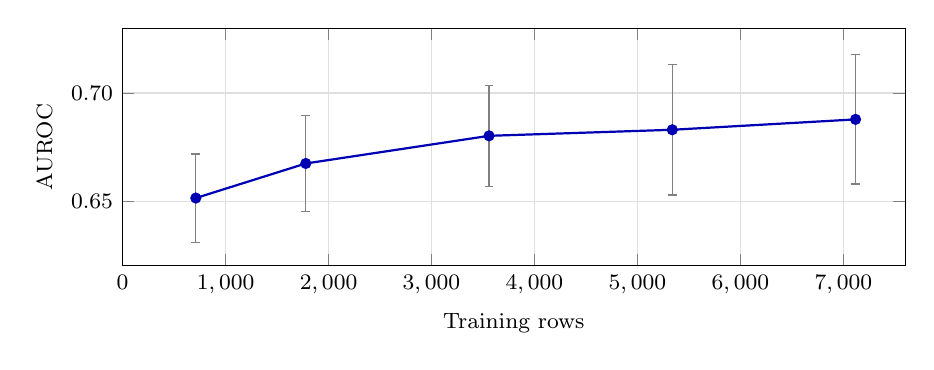
\begin{tikzpicture}
\begin{axis}[width=0.95\columnwidth, height=4.6cm, xlabel={Training rows}, ylabel={AUROC},
  xmin=0, xmax=7600, ymin=0.62, ymax=0.73, label style={font=\footnotesize}, ticklabel style={font=\footnotesize},
  yticklabel style={/pgf/number format/fixed, /pgf/number format/fixed zerofill, /pgf/number format/precision=2},
  scaled x ticks=false, xticklabel style={/pgf/number format/1000 sep={,}}, grid=major, grid style={gray!25}]
\addplot[blue!70!black, thick, mark=*, mark size=1.6pt, error bars/.cd, y dir=both, y explicit, error bar style={gray}] coordinates {(711,0.6514) +- (0,0.0204) (1779,0.6674) +- (0,0.0222) (3559,0.6802) +- (0,0.0233) (5339,0.6830) +- (0,0.0302) (7119,0.6878) +- (0,0.0299)};
\end{axis}
\end{tikzpicture}

\caption{Learning curve over the same ten folds (mean $\pm$ fold std.).}
\label{fig:curve}
\end{figure}

Meanwhile inference latency spans three orders of magnitude (0.2 to
195.0\,$\mu$s per row) and serialized model size spans 0.9\,KB to 63.4\,MB
(Table~\ref{tab:nine}), for 0.031 AUROC (Fig.~\ref{fig:latency}); the rational
choice is the cheapest model not significantly worse.

\begin{figure}[t]
\centering
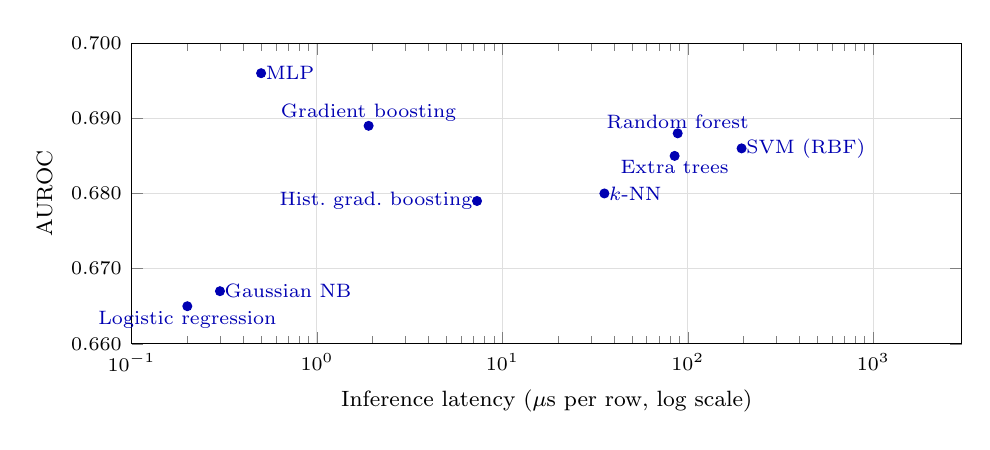
\begin{tikzpicture}
\begin{semilogxaxis}[
  width=\columnwidth, height=5.4cm,
  xmin=0.1, xmax=3000, ymin=0.660, ymax=0.700,
  xlabel={Inference latency ($\mu$s per row, log scale)},
  ylabel={AUROC},
  label style={font=\footnotesize}, ticklabel style={font=\scriptsize},
  yticklabel style={/pgf/number format/fixed, /pgf/number format/fixed zerofill, /pgf/number format/precision=3},
  grid=major, grid style={gray!25},
  nodes near coords, point meta=explicit symbolic,
  every node near coord/.style={font=\scriptsize, inner sep=1.5pt}]
\addplot[only marks, mark=*, mark size=1.6pt, blue!70!black,
  visualization depends on={value \thisrow{anc}\as\anc},
  every node near coord/.append style={anchor=\anc}]
  table[x=lat, y=auc, meta=name]{
  lat   auc   name                    anc
  0.5   0.696 MLP                     west
  1.9   0.689 {Gradient boosting}     south
  88.2  0.688 {Random forest}         south east
  195.0 0.686 {SVM (RBF)}             west
  84.9  0.685 {Extra trees}           north east
  35.5  0.680 {$k$-NN}                west
  7.3   0.679 {Hist.\ grad.\ boosting} east
  0.3   0.667 {Gaussian NB}           west
  0.2   0.665 {Logistic regression}   north west
  };
\end{semilogxaxis}
\end{tikzpicture}
\caption{AUROC against inference latency (log scale). Three orders of
magnitude of latency buy 0.031 AUROC.}
\label{fig:latency}
\end{figure}

\section{Deep Learning: Calibrating Identity}
Face detection uses SCRFD~\cite{guo2022} and embedding uses
\mbox{ArcFace}~\cite{deng2019}; both are frozen. Retraining on project-scale data
would be worse and would introduce demographic bias we cannot audit. The vendor
pack's age and gender classifier is excluded by a loader allow-list.

The system originally used an authored cosine-similarity threshold of 0.50,
reasoned and documented but flagged as uncalibrated. An equal-error-rate sweep
on 2,200 LFW~\cite{huang2007} training pairs, evaluated on 1,000 held-out
pairs, gives Table~\ref{tab:face}; the embedding's AUC on the held-out pairs
is 0.9785 at any threshold.

\begin{table}[t]
\caption{Face-Verification Threshold Before and After Calibration
(LFW, 1,000 Held-Out Pairs)}
\label{tab:face}
\centering
\footnotesize
\begin{tabular}{@{}lccc@{}}
\toprule
Threshold & FAR & FRR & Acc. \\
\midrule
\textbf{0.1266} (calibrated) & 0.030 & \textbf{0.034} & \textbf{0.968} \\
0.50 (authored)              & 0.000 & 0.414 & 0.793 \\
\bottomrule
\end{tabular}
\end{table}

The authored value would have falsely rejected 41.4\% of genuine matches.
Because the system correctly refuses to treat an unmeasured check as a pass,
roughly two in five legitimate candidates would have accumulated integrity
flags for being themselves. Calibration cut false rejection twelvefold at a
false-acceptance cost of 3.0\%. In security-adjacent systems, \emph{reasoned}
and \emph{correct} are different properties, and only one can be demonstrated.

The identity result type is three-valued. \code{Unchecked} carries a reason and
has no similarity field at all---not 0.0, not null---so no downstream
comparison can read a failed measurement as a low-but-real one, in the spirit
of distribution-free abstention~\cite{vovk2005}. LFW is a public-figure
benchmark, not our candidate population; population-specific recalibration
requires consented candidate data we have not collected.

\begin{table*}[t]
\caption{Mapping Regulatory Obligations Onto Architectural Mechanisms}
\label{tab:reg}
\centering
\footnotesize
\begin{tabular}{@{}p{0.17\textwidth}p{0.27\textwidth}p{0.48\textwidth}@{}}
\toprule
Obligation & Instrument & Mechanism in CogniHire \\
\midrule
Bias audit of the tool & NYC Local Law 144~\cite{nycll144} & No composite score to audit; the audited object is the per-claim verdict distribution \\
Candidate notification & NYC Local Law 144~\cite{nycll144}; Illinois AI Video Interview Act~\cite{ilaivia}; Illinois HB 3773~\cite{ilhb3773} & Consent captured per session with a recorded consent version \\
Human oversight & EU AI Act, Art.~14 (high-risk systems; employment is listed in Annex III)~\cite{euaiact} & Report generation is a deterministic transform containing no code that could emit a recommendation \\
Explanation of decisions & EU AI Act, Art.~86~\cite{euaiact} & Every verdict carries its evidence and character offsets into the candidate's own words \\
Non-discrimination & Illinois Human Rights Act as amended by HB 3773~\cite{ilhb3773} & No demographic inference, no outcome labels, no historical decision pattern to inherit \\
Record-keeping & EU AI Act, Art.~12~\cite{euaiact} & Append-only event store; sessions reconstructible turn by turn \\
\bottomrule
\end{tabular}
\end{table*}

\section{Integration, Compliance, and Limitations}
Each family alone leaves a gap. Grounding guarantees claims are the candidate's
own words but not that a session gathered enough evidence to judge them; ML
measures evidence sufficiency but, without grounding, would measure text a
model may have invented; DL supplies identity continuity but no verdict.
Together they close a loop that terminates in a human reviewer, not an
aggregate.

This design maps directly onto regulation (Table~\ref{tab:reg}). The
instruments share a direction: an automated employment decision must be
disclosed, auditable, and open to human oversight and explanation. A system architected around a scalar faces a
retrofit its own architecture resists, since the explanatory information was
discarded at design time. The mapping in Table~\ref{tab:reg} is possible only
because CogniHire declines to produce an aggregate: a bias audit of a composite
score must explain the score, whereas a bias audit of a claim audit examines
the distribution of verdicts and the evidence attached to each---a smaller and
better-posed question.

\emph{Lessons from a reference implementation.} Before building, we audited a
comparable open system in full. Its computer-vision core was sound, but its
decision layer was largely fabricated. An object detector configured with an
invalid model name never ran once; a luminance heuristic filled the gap and
logged window glare as \emph{camera-verified} phone detections, which fed an
escalating penalty system, while a status string reading \emph{engine ready}
was never rendered anywhere. The identity endpoint returned a 0.98-confidence
match when no enrolled face existed at all, and a r\'esum\'e analyzer returned
a hardcoded skill list on zero keyword matches. The defects share one root
cause: a fallback that fabricates a measurement is worse than an outage.
CogniHire's responses---a value-free type for failed measurements, component
health surfaced to a human, every output traceable to a source span---follow
directly. For the same reason we deliberately do \emph{not} build affect,
stress, or deception estimation: none has defensible ground truth on a diverse
candidate pool, and a stress percentage that silently changes which questions
a candidate is asked is itself a hidden score.

\emph{Limitations.} We state three gaps openly. Identity matching is
implemented and tested but is currently only a presence gate on the production
path, so continuous identity verification is not yet deployed. The face
threshold is calibrated on a public benchmark, not candidates. And no
structured recruiter validation study has been conducted, so the premise that
reviewers prefer a claim audit to a score is untested; a controlled comparison
measuring inter-reviewer agreement is the most valuable next study. Finally, a
r\'esum\'e--posting fit model from an earlier iteration of this work (0.657
AUROC) is deliberately not deployed: Section~\ref{sec:within} shows that
pooled fit scores on this benchmark largely reward ranking candidates rather
than matching them.

\section{Conclusion and Future Work}
CogniHire replaces the composite hiring score with a per-claim audit whose
guarantees are enforced by architecture rather than by prompt discipline.
Three findings stand out. The grounding gate rejected every meaning-preserving
paraphrase and negation trap across ${\sim}$100,000 trials while admitting
every verbatim claim. A carefully reasoned similarity constant would have
falsely rejected 41.4\% of genuine identity matches; measurement reduced that
to 3.4\%. And nine classifiers proved statistically indistinguishable at the
top of a public screening benchmark, while a within-query diagnostic showed
that the pooled metric's apparent gains came from ranking candidates rather
than matching them. That last finding overturned our own initial hypothesis;
we report the sequence because a diagnostic proves its power only when it
refutes something.

Three steps follow directly from the limitations in Section~VII: a controlled
recruiter study comparing inter-reviewer agreement on a claim audit against a
composite score; recalibration of the face threshold on consented candidate
data; and continuous identity verification on the production path.

\section*{Data Availability}
Analysis code, per-fold results, and figure sources are available from the
author on request. % AUTHOR: replace with a public repository URL or DOI if you have one.
The face study uses the public LFW benchmark and the grounding evaluation a
synthetic corpus; no human subjects were involved.

\balance
\begin{thebibliography}{99}

\bibitem{raghavan2020}
M.~Raghavan, S.~Barocas, J.~Kleinberg, and K.~Levy, ``Mitigating bias in
algorithmic hiring: Evaluating claims and practices,'' in \emph{Proc. Conf.
Fairness, Accountability, and Transparency (FAT* '20)}, Barcelona, Spain,
2020, pp.~469--481.

\bibitem{dacrema2019}
M.~Ferrari Dacrema, P.~Cremonesi, and D.~Jannach, ``Are we really making much
progress? A worrying analysis of recent neural recommendation approaches,'' in
\emph{Proc. 13th ACM Conf. Recommender Systems (RecSys '19)}, Copenhagen,
Denmark, 2019, pp.~101--109.

\bibitem{musgrave2020}
K.~Musgrave, S.~Belongie, and S.-N. Lim, ``A metric learning reality check,''
in \emph{Computer Vision -- ECCV 2020}, ser. LNCS, vol.~12370. Cham,
Switzerland: Springer, 2020, pp.~681--699.

\bibitem{grinsztajn2022}
L.~Grinsztajn, E.~Oyallon, and G.~Varoquaux, ``Why do tree-based models still
outperform deep learning on typical tabular data?'' in \emph{Advances in
Neural Information Processing Systems (NeurIPS), Datasets and Benchmarks
Track}, 2022.

\bibitem{demsar2006}
J.~Dem\v{s}ar, ``Statistical comparisons of classifiers over multiple data
sets,'' \emph{J. Mach. Learn. Res.}, vol.~7, pp.~1--30, 2006.

\bibitem{nadeau2003}
C.~Nadeau and Y.~Bengio, ``Inference for the generalization error,''
\emph{Mach. Learn.}, vol.~52, no.~3, pp.~239--281, 2003.

\bibitem{gorman2019}
K.~Gorman and S.~Bedrick, ``We need to talk about standard splits,'' in
\emph{Proc. 57th Annu. Meeting Assoc. Comput. Linguistics (ACL)}, Florence,
Italy, 2019, pp.~2786--2791.

\bibitem{kapoor2023}
S.~Kapoor and A.~Narayanan, ``Leakage and the reproducibility crisis in
machine-learning-based science,'' \emph{Patterns}, vol.~4, no.~9, Art.
no.~100804, 2023.

\bibitem{guo2022}
J.~Guo, J.~Deng, A.~Lattas, and S.~Zafeiriou, ``Sample and computation
redistribution for efficient face detection,'' in \emph{Proc. Int. Conf.
Learning Representations (ICLR)}, 2022.

\bibitem{deng2019}
J.~Deng, J.~Guo, N.~Xue, and S.~Zafeiriou, ``ArcFace: Additive angular margin
loss for deep face recognition,'' in \emph{Proc. IEEE/CVF Conf. Computer
Vision and Pattern Recognition (CVPR)}, 2019, pp.~4690--4699.

\bibitem{huang2007}
G.~B. Huang, M.~Ramesh, T.~Berg, and E.~Learned-Miller, ``Labeled Faces in the
Wild: A database for studying face recognition in unconstrained
environments,'' Univ. Massachusetts, Amherst, MA, USA, Tech. Rep. 07-49,
Oct. 2007.

\bibitem{cnamuangtoun2024}
cnamuangtoun, ``resume-job-description-fit,'' Hugging Face Datasets, 2024.
[Online]. Available:
\url{https://huggingface.co/datasets/cnamuangtoun/resume-job-description-fit}
(accessed Sep. 24, 2026).

\bibitem{pedregosa2011}
F.~Pedregosa \emph{et al.}, ``Scikit-learn: Machine learning in Python,''
\emph{J. Mach. Learn. Res.}, vol.~12, pp.~2825--2830, 2011.

\bibitem{vovk2005}
V.~Vovk, A.~Gammerman, and G.~Shafer, \emph{Algorithmic Learning in a Random
World}. New York, NY, USA: Springer, 2005.

\bibitem{nycll144}
New York City Council, ``Local Law 144 of 2021: Automated employment decision
tools,'' N.Y.C. Admin. Code \S\S~20-870--20-874, enacted Dec. 2021, enforced
from Jul. 5, 2023.

\bibitem{ilaivia}
Illinois General Assembly, ``Artificial Intelligence Video Interview Act,''
820 ILCS 42, effective Jan. 1, 2020.

\bibitem{ilhb3773}
Illinois General Assembly, ``HB 3773: Amendment to the Illinois Human Rights
Act (artificial intelligence in employment),'' Public Act 103-0804, effective
Jan. 1, 2026.

\bibitem{euaiact}
European Parliament and Council of the European Union, ``Regulation (EU)
2024/1689 laying down harmonised rules on artificial intelligence (Artificial
Intelligence Act),'' \emph{Off. J. Eur. Union}, OJ L, 2024/1689, Jul. 12, 2024.

\end{thebibliography}

\end{document}
